\section{Matrix diffusion}

\subsection{Definition}

This benchmark is introduced to verify the matrix diffusion function. It simulates
advective -dispersive transport of a solute in an one-dimensional
fracture with constant aperture, with and without the effect of
matrix-diffusion. The geometry and the material parameters are
chosen to fit the parameters extracted from experiments conducted
during the Colloid Radionuclide Retardation Experiment at Nagra's
Grimsel test site \cite{KosaSmith:2005}. The result from GS/RF is
compared with that from PICNIC, and they fit well.

\begin{figure}[!htb]
  \begin{center}
    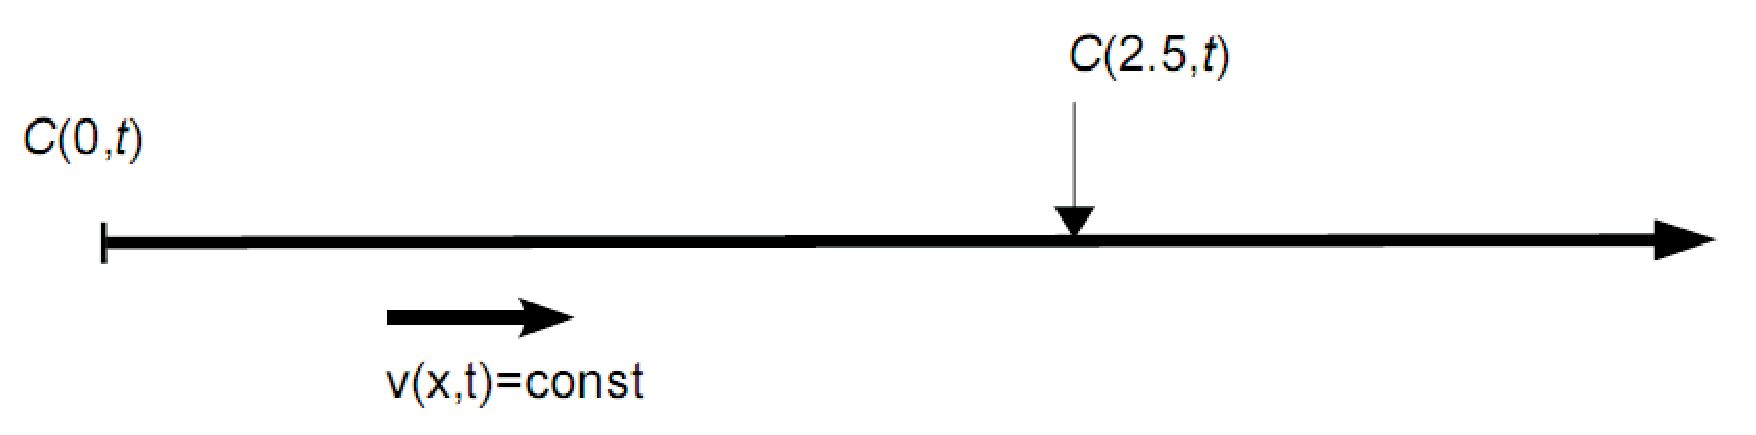
\includegraphics[scale=0.25]{PART_II/C/fig_matdiff_domain.eps}
  \end{center}
  \caption{Conceptual setup of the 1D problem}
  \label{c:matdiff_dom}
\end{figure}

The geometry and material parameters in PICNIC and OGS are
summarized in Table \ref{tab:c_matdiff_setting} and the conceptual
model is shown in Figure \ref{c:matdiff_dom}. PICNIC solves the
one-dimensional problem, whereas in OGS a two-dimensional
discretization was chosen. A rectangular domain of 5.2m $\times$
0.5m was discretized with 1155 nodes and 2080 triangular elements.
One of the shorter domain edges was chosen as inflow boundary and
fluid was injected at the boundary-nodes in such a way, that the
resulting fluid velocity matches exactly the value from Table
\ref{tab:c_matdiff_setting}. The concentration is fixed at the
inflow boundary. In 2.5m distance the breakthrough curve is
recorded. The outflow boundary is assumed to be far away and should
not influence the observed breakthrough curve.Picnic V2.2 and OGS (Rev. 1535).

As defining exactly the same transport boundary conditions in OGS
and PICNIC is not possible, the following procedure was used to get
the inflow boundary condition as similar as possible:

\begin{enumerate}
	\item 
The system was calculated for injecting a pulse of solute with a
constant flux for a time length of 50s with PICNIC. The
concentration vs. time was recorded for the inflow-leg.
  \item
The concentrations vs. time extracted from PICNIC's inflow-leg
were applied (fixed) to the inflow boundary of the OGS system.
\end{enumerate}

These procedures work, as long as advective fluxes are much higher
than the dispersive-diffusive fluxes over the boundary.
%
The outflow boundary condition is set to infinity, i.e. a
semi-infinite problem is calculated. In OGS the domain is set to
5m, double the distance between inflow boundary and observation
point. This prevents the outflow boundary condition to influence the
tracer breakthrough at the observation point.

\begin{table}[htb]%[tab-ldhp]
\begin{center}
\begin{tabular}{llrr}
\toprule
Symbol & Parameter & Value & Unit \\
\midrule
 $L$ & Distance between boundary & & \\
     & and observation points & $2.5$ & $m$ \\
 $\alpha_{T}$ & Transverse dispersion (OGS only) & $-$ & $m$ \\
 $\rho$ & Bulk matrix density & $2670$ & $kg/m^{3}$ \\
 $2b$ & Fracture aperture & $0.55\times10^{-3}$ & $m$ \\
 $v$ & Fluid velocity & $7.05\times10^{-4}$ & $m/s$ \\
 $\alpha_{L}$ & Longitudinal dispersion (OGS only) & $0.1$ & $m$ \\
 $Pe$ & Peclet number (PICNIC only) & $25$ & $-$ \\
 $\varepsilon_{p}$ & Matrix porosity & $0.3$ & $-$ \\
 $D_{p}$ & Diffusion constant in rock matrix & $7.4\times10^{-11}$ & $m^{2}/s$ \\
\bottomrule
\end{tabular}
\caption{Geometry and material properties for the simulations} %\footnotesize
\label{tab:c_matdiff_setting}
\end{center}
\end{table}

\subsection{Results}

For the investigated two cases, advection and dispersion(ADE) only
and ADE plus matrix diffusion(MD), the PICNIC and OGS solutions
are in general very similar (see Figure \ref{c:matdiff_result}).

\begin{figure}[!htb]
  \begin{center}
  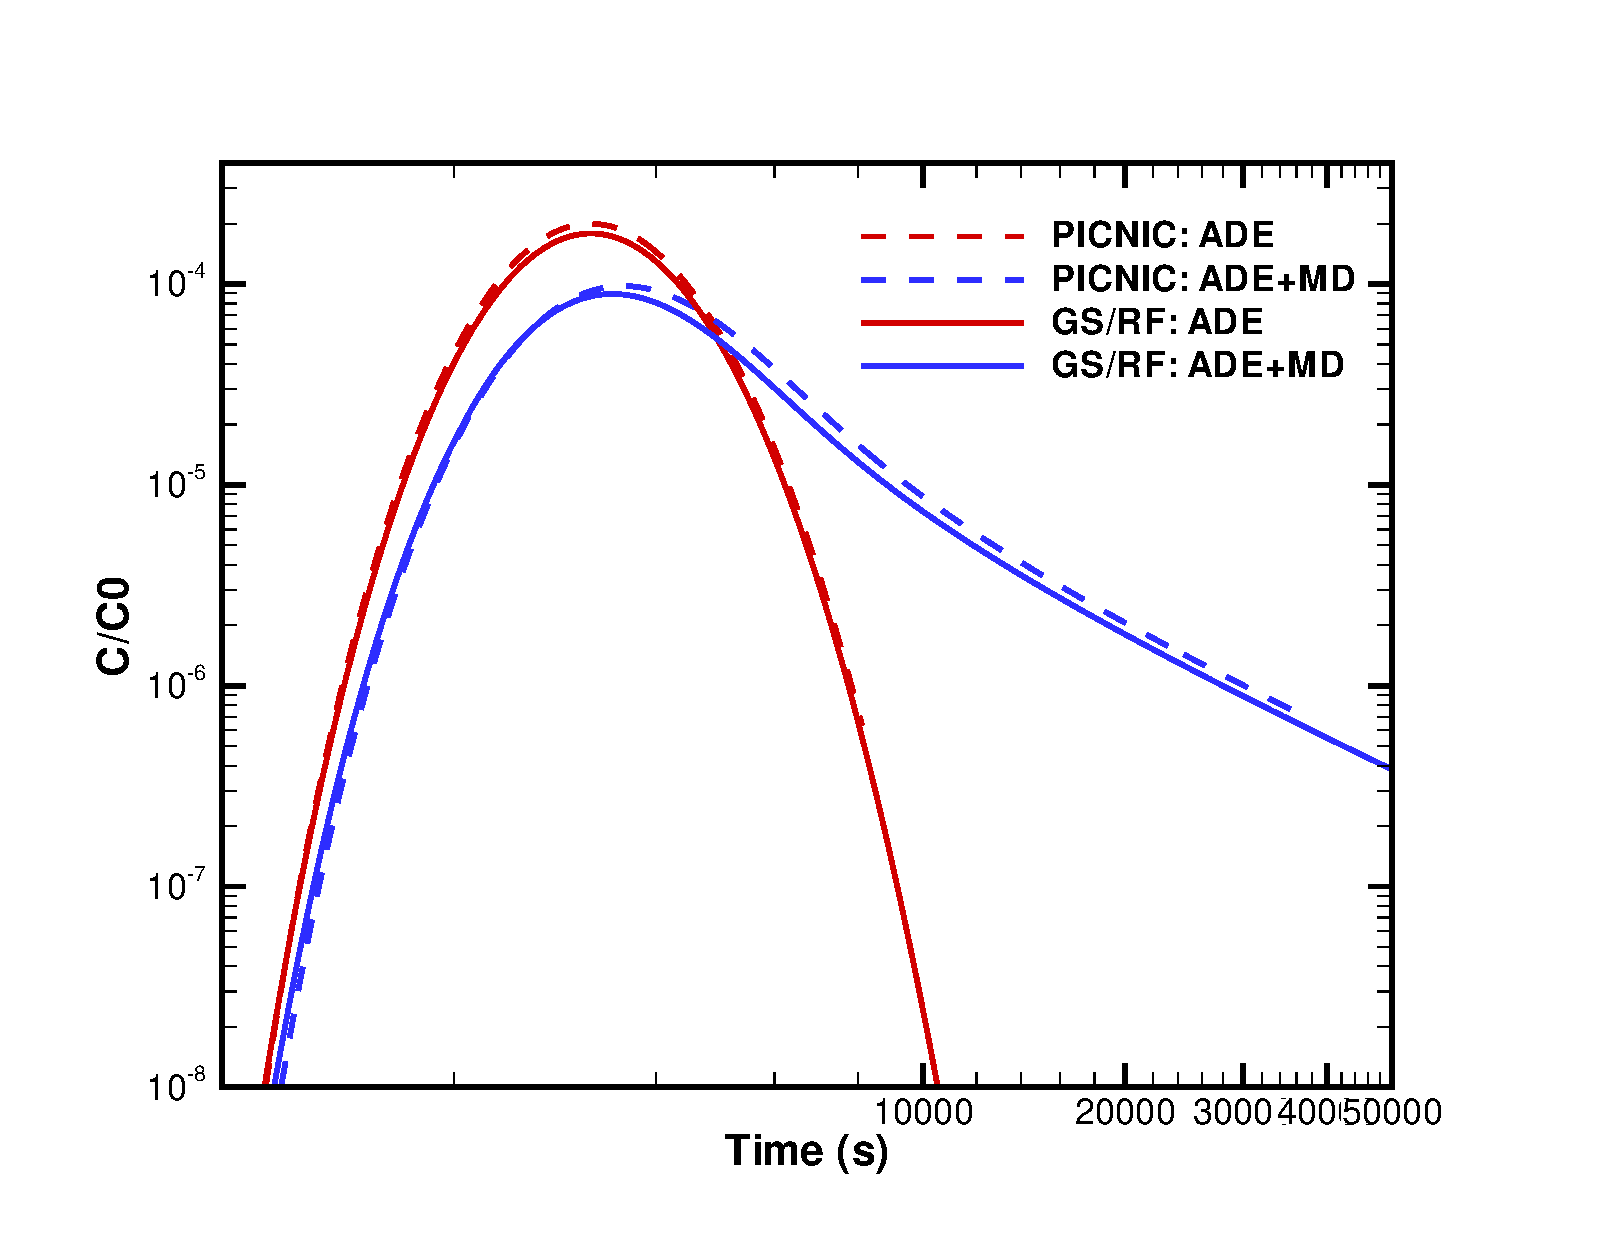
\includegraphics[scale=0.4]{PART_II/C/fig_matdiff_result.eps}
  \end{center}
  \caption{Breakthrough of the ADE and the ADE+MD solutions calculated with PICNIC and OGS}
  \label{c:matdiff_result}
\end{figure}

\newpage